\documentclass[aspectratio=1610,onlymath]{beamer}
% \documentclass[aspectratio=1610,onlymath,handout]{beamer}

\input{macros-lecture}
% Common notation

\usepackage{amsmath,amssymb,amsfonts}
\usepackage{xspace}

\newcommand{\lectureurl}{https://iccl.inf.tu-dresden.de/web/FS2023}

\DeclareMathAlphabet{\mathsc}{OT1}{cmr}{m}{sc} % Let's have \mathsc since the slide style has no working \textsc

% Dual of "phantom": make a text that is visible but intangible
\newcommand{\ghost}[1]{\raisebox{0pt}[0pt][0pt]{\makebox[0pt][l]{#1}}}

\newcommand{\tuple}[1]{\langle{#1}\rangle}
\newcommand{\defeq}{\mathrel{:=}}

%%% Annotation %%%

\usepackage{color}
\newcommand{\todo}[1]{{\tiny\color{red}\textbf{TODO: #1}}}



%%% Old macros below; move when needed

\newcommand{\blank}{\text{\textvisiblespace}} % empty tape cell for TM

% table syntax
\newcommand{\dom}{\textbf{dom}}
\newcommand{\adom}{\textbf{adom}}
\newcommand{\dbconst}[1]{\texttt{"#1"}}
\newcommand{\pred}[1]{\textsf{#1}}
\newcommand{\foquery}[2]{#2[#1]}
\newcommand{\ground}[1]{\textsf{ground}(#1)}
% \newcommand{\foquery}[2]{\{#1\mid #2\}} %% Notation as used in Alice Book
% \newcommand{\foquery}[2]{\tuple{#1\mid #2}}

\newcommand{\quantor}{\mathord{\reflectbox{$\text{\sf{Q}}$}}} % the generic quantor

% logic syntax
\newcommand{\Inter}{\mathcal{I}} %used to denote an interpretation
\newcommand{\Jnter}{\mathcal{J}} %used to denote another interpretation
\newcommand{\Knter}{\mathcal{K}} %used to denote yet another interpretation
\newcommand{\Zuweisung}{\mathcal{Z}} %used to denote a variable assignment

% query languages
\newcommand{\qlang}[1]{{\sf #1}} % Font for query languages
\newcommand{\qmaps}[1]{\textbf{QM}({\sf #1})} % Set of query mappings for a query language

%%% Complexities %%%

\hyphenation{Exp-Time} % prevent "Ex-PTime" (see, e.g. Tobies'01, Glimm'07 ;-)
\hyphenation{NExp-Time} % better that than something else

% \newcommand{\complclass}[1]{{\sc #1}\xspace} % font for complexity classes
\newcommand{\complclass}[1]{\ensuremath{\mathsc{#1}}\xspace} % font for complexity classes

\newcommand{\ACzero}{\complclass{AC$_0$}}
\newcommand{\LogSpace}{\complclass{L}}
\newcommand{\NLogSpace}{\complclass{NL}}
\newcommand{\PTime}{\complclass{P}}
\newcommand{\NP}{\complclass{NP}}
\newcommand{\coNP}{\complclass{coNP}}
\newcommand{\PH}{\complclass{PH}}
\newcommand{\PSpace}{\complclass{PSpace}}
\newcommand{\NPSpace}{\complclass{NPSpace}}
\newcommand{\ExpTime}{\complclass{ExpTime}}
\newcommand{\NExpTime}{\complclass{NExpTime}}
\newcommand{\ExpSpace}{\complclass{ExpSpace}}
\newcommand{\TwoExpTime}{\complclass{2ExpTime}}
\newcommand{\NTwoExpTime}{\complclass{N2ExpTime}}
\newcommand{\ThreeExpTime}{\complclass{3ExpTime}}
\newcommand{\kExpTime}[1]{\complclass{#1ExpTime}}
\newcommand{\kExpSpace}[1]{\complclass{#1ExpSpace}}


\defineTitle{1}{Willkommen/Einleitung formale Sprachen}{9. Oktober 2023}
% \defineTitle{1}{Willkommen}{26. Oktober 2020}

\begin{document}

\maketitle


\sectionSlide{Willkommen zur Vorlesung\\Formale Systeme}

% \begin{frame}\frametitle{}
% 
% ~\hfill
% \includegraphics[height=6.5cm]{a1}
% \hfill~
% 
% \end{frame}

\begin{frame}\frametitle{Raum, Zeit, URL}

\begin{itemize}
\item \emph{Vorlesungstermine:}\\
	Montag, DS3 (11:10--12:40)\\
	Donnerstag, DS4 (13:00--14:30)
\item \emph{Videos:}\\
	frei verfügbar für alle Vorlesungstermine:\\
	\url{https://www.youtube.com/channel/UC0mGxSeFgs3iCNPrypD4Z5g/}\\
	(siehe Playlists)
% \item \emph{Keine Vorlesungen:}\\
% 	\redalert{Mo 23.10.}\\
% 	Jahreswechsel: Do 21.12., Mo 25.12., Do 28.12., Mo 1.1.
\item \emph{Vorlesungswebseite}:\\[.5ex]
	\url{\lectureurl}\\[0.5ex]
	{\footnotesize(Folien, Übungsblätter, Termine, etc.)}
\item \emph{Quellen, Bug-Reports, Fragen}:\\[.5ex]
	\url{https://github.com/knowsys/FormaleSysteme}\\[.5ex]
	{\footnotesize(Pull-Requests sind willkommen)}
\item \emph{Chatkanal (Matrix)}\\[.5ex]
	\url{https://matrix.tu-dresden.de/\#/room/\#fosys:tu-dresden.de}
% \item \emph{Mailingliste}:\\[0.5ex]
% \footnotesize
% 	\url{https://mailman.zih.tu-dresden.de/groups/listinfo/inf-thi-fs1718}\\[0.5ex]
% 	{\footnotesize(Support bei allen Fragen zur Vorlesung)}
\end{itemize}

\end{frame}


\begin{frame}\frametitle{Übungen}
\begin{itemize}
\item \emph{Anmeldung} zu den Übungen über OPAL (Link siehe Vorlesungswebseite)
\item \emph{Übungsblätter} jeweils montags ``nach der Vorlesung''\\
	(erstes Übungsblatt am 9. Oktober 2023)
\item \emph{Beginn der Übungen:} 16. Oktober 2023
\item \emph{Übungsablauf}, vereinfacht, idealisiert:\\
	Aufgaben werden zu Hause bearbeitet so gut es geht;\\
	in der Übung helfen Gruppenleiter/innen bei Fragen und Problemen und zeigen Beispiellösungen\\[1ex]
\end{itemize}

\end{frame}


\begin{frame}\frametitle{Prüfung und Prüfungsvorbereitung}
\begin{itemize}
\item schriftliche Prüfung (90min) am Ende des Wintersemesters
\item prüfungsrelevant:\\
	kompletter Stoff, der in der Vorlesung und Übung behandelt wird\\
	Wiedergeben (Definieren) \alert{und} Anwenden (Rechnen)
\item Modulnote ergibt sich je nach Studiengang
\item zur zusätzlichen Vorbereitung wird es eine Probeklausur geben
% gibt es \alert{2--3 Repetitorien} und \alert{eine Probeklausur}, jeweils an einem Vorlesungstermin
\end{itemize}

\end{frame}


\begin{frame}\frametitle{Formale Systeme Bestehen}
Tipps:
\begin{itemize}
\item \emph{Von Hand Mitschreiben}\\
	{\footnotesize Man merkt sich Stoff deutlich besser, wenn man ihn für sich selbst handschriftlich
	zusammenfasst.\footnote{\tiny P.\ Mueller \& D.\ Oppenheimer. The Pen Is Mightier Than the Keyboard: Advantages of Longhand Over Laptop Note Taking. Psychological Science, 06/2014, 25:6}}
\item \emph{Selber Rechnen}\\
	{\footnotesize Die Prüfung besteht im Lösen von Rechenaufgaben. Theorie allein hilft da nicht weiter.}
\item \emph{Schnell sein}\\
	{\footnotesize Prüfungszeit ist meistens knapp. Es reicht nicht, Aufgaben "`im Prinzip"' lösen zu können. Man muss sie schnell lösen.}
\item \emph{Ehrlich zu sich selbst sein}\\
	{\footnotesize Man sollte selbst wissen, ob man genug gelernt hat oder nicht.\footnote{\tiny Vgl.\ aber auch Wikipedia \href{https://de.wikipedia.org/wiki/Dunning-Kruger-Effekt}{[[Dunning-Kruger-Effekt]]}}}
\end{itemize}

\end{frame}


\sectionSlide{Übersicht und Motivation}

\newcommand{\qaline}[2]{\alert{#1}\\\hfill\pause \textcolor{darkred}{#2}\\[1.5ex]}

% Uebersicht Thema und Ziel der Vorlesung,
\begin{frame}\frametitle{Grundlegende Fragen der Informatik}

\qaline{Was ist ein Computer?}{Eine Maschine, die rechnet.}\pause

\qaline{Was ist "`Rechnen"'?}{Die systematische Überführung von Eingaben in Ausgaben.}\pause

\qaline{Was sind "`Eingaben"' und "`Ausgaben"'?}{Folgen von Zeichen, zum Beispiel Dateien oder Textausgaben.}\pause

\qaline{So viele Computer, Programme, \ldots{} das passt doch in kein \ghost{Studium!}}{Nein, man muss sich auf das Wesentliche konzentrieren.}\pause
% Mit Hilfe von Modellen für Computer und Rechenverfahren.\\[1ex]

\qaline{Was ist das Wesentliche?}{Vereinfachte Modelle für Computer und Rechenverfahren.}\pause

\qaline{Was sagen uns Modelle über echte Computer und Software?}{Was man berechnen kann, wie aufwändig es ist,\\\hfill wie man es implementieren kann, ob es stimmt, \ldots}

\end{frame}


\begin{frame}\frametitle{Zielstellung, Kernthemen}

Ziel dieser Vorlesung ist es, wichtige Grundlagen zur \alert{Modellierung von Berechnung}
in der Informatik einzuführen, \alert{konkrete Modelle} vorzustellen und ihre \alert{Eigenschaften verständlich zu machen}.
\medskip

\begin{itemize}
\item Ein- und Ausgaben sind Zeichenfolgen\\
$\leadsto$ Wir beginnen mit Wörtern und \redalert{formalen Sprachen}
%
\item Wir wollen Berechnungsaufgaben beschreiben\\
$\leadsto$ Spezifikation von Sprachen\\
\hspace{1em} (direkt, mit \redalert{Grammatiken}, mit \redalert{regulären Ausdrücken}, \ldots)
%
\item Fokus auf einfache Berechnungsmodelle\\
$\leadsto$ \redalert{Automaten} (in vielen Versionen \ldots)
%
\item Man kann Berechnungsaufgaben auch logisch spezifizieren\\
$\leadsto$ \redalert{Aussagenlogik} als einfacher Einstieg
%
\item Lösung logischer Probleme\\
$\leadsto$ Berechnungsverfahren zum \redalert{logischen Schließen}
\end{itemize}

\end{frame}


\begin{frame}\frametitle{Gliederung "`Formale Systeme"'}

\alert{Teil 1: Sprachen und Automaten}
\begin{itemize}
\item Formale Sprachen und Grammatiken
\item Reguläre Sprachen und endliche Automaten
\item Kontextfreie Sprachen und Kellerautomaten
\item Kontextsensitive Sprachen, Typ-0-Sprachen und \ghost{Turingmaschinen}
\end{itemize}
\bigskip

\alert{Teil 2: Aussagenlogik}
\begin{itemize}
\item Syntax und Semantik
\item logisches Schließen, Backtracking und andere Verfahren
\item Horn-Logik als Vereinfachung
\end{itemize}

\end{frame}

% \overviewslide

\begin{frame}\frametitle{Literatur: Lehrbücher}

Der Vorlesungsstoff gehört zu fast jeder Informatikausbildung. Es gibt viele
Lehrmaterialien und eine weitgehend einheitliche \ghost{Notation.}
\bigskip

Lehrbücher zum ersten Teil der Vorlesung (formale Sprachen):

\begin{itemize}
\item Uwe Schöning: \emph{Theoretische Informatik -- kurz gefasst.} Spektrum Akademischer Verlag\\
{\footnotesize\textcolor{devilscss}{deutschsprachiger Standardtext; in der Tat ziemlich kurz gefasst}}
%
\item John E. Hopcroft, Rajeev Motwani, Jeffrey D. Ullman: \emph{Einführung in Automatentheorie, Formale Sprachen und Berechenbarkeit.} Pearson Studium\\
{\footnotesize\textcolor{devilscss}{aus dem Englischen übertragenes Standardwerk; Original ev. besser}}
%
\item Michael Sipser: \emph{Introduction to the Theory of Computation.}  Cengage Learning\\
{\footnotesize\textcolor{devilscss}{Standardtext zu Sprachen und Berechnungskomplexität; leider nur auf Englisch}}
\end{itemize}

\end{frame}

\begin{frame}\frametitle{Literatur: Frei zugängliche Skripte}

Es existieren mehrere Skripte zu dieser Vorlesung:
\begin{itemize}
\item Franz Baader: \emph{Skript Formale Systeme, Teil 1 -- Automaten und formale Sprachen.} TU Dresden.
\\{\tiny Siehe \url{https://lat.inf.tu-dresden.de/teaching/ws2013-2014/FS/script_2016-02.pdf}}.
\item Christel Baier, Manuela Berg, Walter Nauber: \emph{Formale Systeme WS 2011/2012: Skript zur Vorlesung.} TU Dresden.
\\{\tiny Leider nicht mehr online. Sachdienliche Hinweise sind willkommen.}
%  \\{\tiny Siehe \url{http://www.inf.tu-dresden.de/content/institutes/thi/algi/lehre/WS1415/FS/lecture_notes/Skript_FS_C_Baier_WS1112.pdf}}.
\end{itemize}

Die Vorlesungen haben kleine Abweichungen, stimmen aber in vielen wichtigen Punkten überein.

\end{frame}

\sectionSlide{Fragen, Ideen, Anmerkungen}



\sectionSlide{Sprachen in der Informatik}


\begin{frame}\frametitle{Wozu Sprachen?}

\end{frame}

\begin{frame}\frametitle{}

~\hfill
\includegraphics[height=8.5cm]{images/xkcd-regexps}
\hfill~
\rotatebox{90}{\tiny Randall Munroe, \url{http://xkcd.com/208/}, CC-BY-NC 2.5}

\end{frame}


\begin{frame}[fragile]\frametitle{Wozu Sprachen?}
\newcommand{\smaller}[1]{{\footnotesize #1}}

Formale Sprachen und die zugehörigen Automaten und Grammatiken haben sehr viele Anwendungen:

\begin{itemize}
\item \alert{Compilerbau}\\
	\smaller{Programmiersprachen sind typische formale Sprachen}
\item \alert{Interpretation natürlicher Sprachen}\\
	\smaller{viele Anwendungen des Sprachverstehens nutzen Grammatiken}
\item \alert{Datenaustausch}\\
	\smaller{Textformate (HTML, CSV, JSON, XML, \ldots) bilden formale Sprachen}
\item \alert{Formatierung/Validierung/Spezifikation}\\
	\smaller{z.B. um die Gültigkeit von Formulareingaben zu prüfen}
\item \alert{Berechenbarkeit und Komplexität}\\
	\smaller{mächtigere Sprachdefinitionen verlangen teurere Algorithmen}
\item \alert{Informationsextraktion}\\
	\smaller{Formale Sprachen helfen bei der Mustersuche in Textdokumenten}
\item \alert{Datenbanken}\\
	\smaller{Datenbankanfragen können Muster suchen, z.B. in \ghost{Graphdatenbanken}}
\end{itemize}

\end{frame}


\begin{frame}[t,fragile]\frametitle{Beispiel Compiler}

\begin{tikzpicture}[
	decoration=penciline, decorate,
	node distance = 7mm and 9mm,
	mybox/.style args = {#1/#2}{
		draw=#1,% line color
		fill=#2,% fill color
% 		rounded corners,
		thick,
		text width=47mm, minimum height=8mm, inner sep=1mm, 
		align=flush center
	},
	myarrow/.style args = {#1}{
		line width=0.8mm,
		draw=#1,%line color
		%-{Triangle[length=2.8mm,width=4mm,fill=#1]},
		->,
		shorten >=0.5mm, shorten <=0.1mm
	},
	myarrowb/.style args = {#1}{
		line width=0.3mm,
		draw=#1,%line color
		%-{Triangle[length=2.8mm,width=4mm,fill=#1]},
		->,
		shorten >=1mm, shorten <=0.1mm
	}
]
\pgfmathsetseed{7729}
% \draw[help lines] (0,0) grid (5,5);
\node (n1) [decorate,mybox=black/cyan!40] at (0,6) {Quellprogramm};
\uncover<1>{
	\node at (0,3) {{\Huge ?}};
}
\uncover<2>{
\node (n2) [decorate,mybox=black/white] at (0,4.5) {Lexer};
	\node (t2) [right=of n2,align=left] {\alert{lexikalische Analyse}\\erzeugt Folge von Tokens\\(${}={}$Bedeutungseinheiten)};
\node (n3) [decorate,mybox=black/white] at (0,3) {Parser};
	\node (t3) [right=of n3,align=left] {\alert{syntaktische Analyse}\\erzeugt Strukturbaum};
\node (n4) [decorate,mybox=black/white] at (0,1.5) {$\ldots$};
	\node (t4) [right=of n4,align=left] {semantische Analyse,\\
	Codeerzeugung,\\Optimierung,\ldots};
}
\node (n5) [decorate,mybox=black/cyan!40] at (0,0) {Programm in Zielsprache};
%
\draw[myarrow=black]    (n1) edge[decorate] (n2);
\uncover<2>{
\draw[myarrow=black]    (n2) edge[decorate] (n3);
\draw[myarrow=black]    (n3) edge[decorate] (n4);
}
\draw[myarrow=black]    (n4) edge[decorate] (n5);
%
\uncover<2>{
\draw[myarrowb=alert]    (t2) edge[decorate] (n2);
\draw[myarrowb=alert]    (t3) edge[decorate] (n3);
\draw[myarrowb=alert]    (t4) edge[decorate] (n4);
}
\end{tikzpicture}

\end{frame}


% Lexer (speziell Scanner)/Parser-Beispiel

\begin{frame}\frametitle{Lexikalische Analyse}

\alert{Eingabe:} Zeichenkette eines Programms\\[1ex]
\examplebox{Bsp.:~~~ $\underbrace{\texttt{\Sterm{lengthCm = lengthInch * 2.54;}}}_{\text{Kette von 29 Zeichen}}$}
% 	\bigskip

\alert{Ausgabe:} Kette von Grundsymbolen (Tokens)\\[1ex]
\examplebox{Bsp.:~~~ $\underbrace{\textsf{\Snterm{NAME EQUALS NAME STAR NUMBER SEMICOLON}}}_{\text{Kette von 6 Tokens}}$}

\begin{itemize}
\item Zur Weiterverarbeitung wird Tokens oft weitere Information mitgegeben,
	z.B. $\textsf{\Snterm{NAME}} (\texttt{"{}\Sterm{lengthCm}"{}})$ und \ghost{$\textsf{\Snterm{NAME}} (\texttt{"{}\Sterm{lengthInch}"{}})$}
\item Manche Zeichen werden nicht zu Tokens\\(z.B. Leerzeichen, Kommentare)
\end{itemize}

\end{frame}

\begin{frame}\frametitle{Lexikalische Analyse (2)}

Verschiedene Arten von Grundsymbolen:
\begin{itemize}
\item Schlüsselwörter (\texttt{\Sterm{if}}, \texttt{\Sterm{while}}, \texttt{\Sterm{class}}, \ldots)
\item Operatoren (\texttt{\Sterm{=}}, \texttt{\Sterm{+}}, \texttt{\Sterm{{>}{}{>}}}, \ldots)
\item Bezeichner (\texttt{\Sterm{lengthCm}}, \texttt{\Sterm{getLength}}, \texttt{\Sterm{InventoryItem}}, \ldots)
\item Literale (\texttt{\Sterm{2.54}}, \texttt{\Sterm{true}}, \texttt{\Sterm{\squote{}Hello World!\squote}}, \ldots)
\end{itemize}
\medskip

Für einige Grundsymbole gibt es unendlich viele Möglichkeiten
\examplebox{Bsp.: "`Ein Bezeichner ist ein String, der mit einem Buchstaben beginnt und danach nur Buchstaben oder Ziffern enthält."'}
% \\[2ex]

Wie soll ein Lexer das korrekt erkennen?

\end{frame}


\begin{frame}\frametitle{Bezeichner erkennen}
\examplebox{Bsp.: "`Ein Bezeichner ist ein String, der mit einem Buchstaben beginnt und danach nur Buchstaben oder Ziffern enthält."'}

Schematische Darstellung als \alert{Syntaxdiagramm}:

\begin{center}
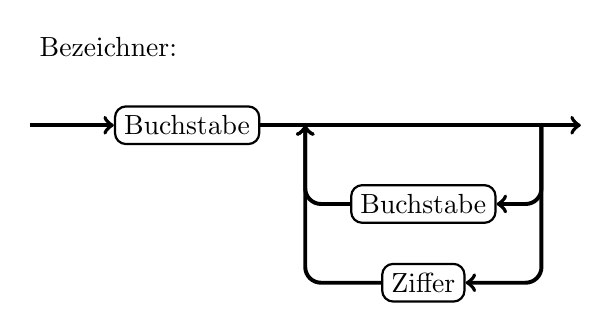
\begin{tikzpicture}
% \draw[help lines] (0,0) grid (7,2);
\node at (0,3) {Bezeichner:};
%
\node (b1) [rounded corners,draw=black,thick] at (1,2) {\Snterm{Buchstabe}};
\node (b2) [rounded corners,draw=black,thick] at (4,1) {\Snterm{Buchstabe}};
\node (z)[rounded corners,draw=black,thick] at (4,0) {\Snterm{Ziffer}};
% \draw[decorate,thick] (0,0) -- (0,3) -- (3,3);
\draw [->,line width=0.5mm] (-1,2) -> (b1);
\draw [->,line width=0.5mm] (b1) -> (6,2);
\draw [->,rounded corners=2mm,line width=0.5mm] (b2) -- (2.5,1) -> (2.5,2);
\draw [->,rounded corners=2mm,line width=0.5mm] (z) -- (2.5,0) -> (2.5,2);
\draw [->,rounded corners=2mm,line width=0.5mm] (5.5,2) -- (5.5,1) -> (b2);
\draw [->,rounded corners=2mm,line width=0.5mm] (5.5,2) -- (5.5,0) -> (z);
\end{tikzpicture}
\end{center}
Hierbei stehen \Snterm{Buchstabe} und \Snterm{Ziffer} jeweils für ein beliebiges Zeichen dieses Typs.

\end{frame}


\newcommand{\nameForInnerLexerState}{inner}

\begin{frame}\frametitle{Bezeichner erkennen (2)}

Wie setzt man das praktisch um?\\
Code eines unerfahrenen Programmierers:\medskip

\codebox{%
{\footnotesize\tt%
\Scode{function} isIdentifier():\\
~~~state = \Sterm{\squote{}start\squote}\\
~~~\Scode{while} hasNextSymbol():\\
~~~~~~~~symbol = getNextSymbol()\\
~~~~~~~~\Scode{if} ( state == \Scodelit{"{}start"{}} \&\& isLetter(symbol) ):\\
~~~~~~~~~~~~~state = \Scodelit{"{}\nameForInnerLexerState"{}}\\
~~~~~~~~\Scode{else if} ( state == \Scodelit{"{}start"{}} \&\& !isLetter(symbol) ):\\
~~~~~~~~~~~~~\Scode{return} \Scodelit{false}\\
~~~~~~~~\Scode{else if} ( state == \Scodelit{"{}\nameForInnerLexerState"{}} \&\& isLetter(symbol) ):\\
~~~~~~~~~~~~~\Scomment{// ok, wir lesen einfach weiter}\\
~~~~~~~~\Scode{else if} ( state == \Scodelit{"{}\nameForInnerLexerState"{}} \&\& isNumber(symbol) ):\\
~~~~~~~~~~~~~\Scomment{// ok, wir lesen einfach weiter}\\
~~~~~~~~\Scode{else if} ( state == \Scodelit{"{}\nameForInnerLexerState"{}} \&\& \\
~~~~~~~~~~~~~~~~~~~~~!isLetter(symbol) \&\& !isNumber(symbol) ):\\
~~~~~~~~~~~~~\Scode{return} \Scodelit{false}\\
~~~\Scode{if} (state == \Scodelit{"{}\nameForInnerLexerState"{}}): \Scode{return} \Scodelit{true}
}}

\end{frame}


\begin{frame}\frametitle{Bezeichner erkennen (3)}

Der (schlechte) Programmcode zeigt eine wichtige Eigenschaft:
\begin{center}
	\redalert{Der Lexer muss nur einen "`Zustand"' speichern}
\end{center}
(im Beispiel ist dies der Wert der Variable \texttt{state})
\bigskip\pause

Darstellung als \alert{endlicher Automat:}\bigskip

\begin{minipage}{5cm}
\doodlebox{gray}{%
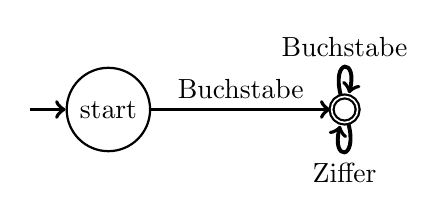
\begin{tikzpicture}
% \draw[help lines] (0,0) grid (7,2);
\node (s1) [circle,draw=black,thick] at (0,0) {start};
\node (s2) [double,circle,draw=black,thick] at (3,0) {\nameForInnerLexerState};
%
\path[->,line width=0.5mm]
(-1,0) edge (s1)
(s1) edge node[above] {\Snterm{Buchstabe}} (s2)
(s2) edge [loop above] node[above] {\Snterm{Buchstabe}} (s2)
(s2) edge [loop below] node[below] {\Snterm{Ziffer}} (s2)
;
\end{tikzpicture}}
\end{minipage}%
% 
\begin{minipage}{6cm}\footnotesize
\begin{itemize}
\item Automat beginnt im Startzustand \scalebox{0.5}{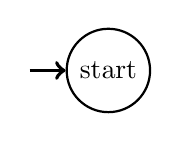
\begin{tikzpicture}[baseline=(s1.base)]\node (s1) [circle,draw=black,thick] at (0,0) {start};\path[->,line width=0.5mm]
(-1,0) edge (s1);\end{tikzpicture}}
\item Zustandswechsel gemäß Pfeilen
\item Kein passender Pfeil für Symbol?\\ "`\texttt{\Scode{return} \Scodelit{false}}"'
\item Keine weiteren Symbole?\\
"`\texttt{\Scode{return} \Scodelit{true}}"' in Endzustand \scalebox{0.5}{
\begin{tikzpicture}[baseline=(s2.base)]\node (s2) [double,circle,draw=black,thick] at (4,0) {\nameForInnerLexerState};\end{tikzpicture}}\\
"`\texttt{\Scode{return} \Scodelit{false}}"' falls in Zustand \scalebox{0.5}{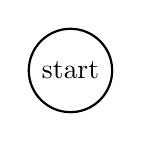
\begin{tikzpicture}[baseline=(s1.base)]\node (s1) [circle,draw=black,thick] at (0,0) {start};
% \path[->,line width=0.5mm](-1,0) edge (s1);
\end{tikzpicture}}
\end{itemize}
\end{minipage}

\end{frame}


\begin{frame}\frametitle{Bezeichner erkennen (4)}

Wie kann man jemandem am besten erklären, was ein "`Bezeichner"' ist?
\begin{itemize}
\item \alert{Sprachliche Umschreibung}: ungenau und mehrdeutig
\item \alert{Syntaxdiagram}, \alert{endlicher Automat}: graphische Darstellung anschaulich, aber schnell unübersichtlich
\item \alert{Programmcode}: Kernidee geht in Implementierungsdetails verloren
\end{itemize}
\pause
$\leadsto$ Spezifikationen verwenden meist \redalert{Grammatiken}

\examplebox{\vspace{-3ex}\begin{align*}
\Snterm{Bezeichner} &\Coloneqq \Snterm{Buchstabe} \mid \Snterm{Buchstabe}~ \Snterm{InBezeichner}\\
\Snterm{InBezeichner} &\Coloneqq \Snterm{BuchOderZiff} \mid \Snterm{BuchOderZiff}~ \Snterm{InBezeichner}\\
\Snterm{BuchOderZiff} &\Coloneqq \Snterm{Buchstabe} \mid \Snterm{Ziffer}\\
\Snterm{Buchstabe} &\Coloneqq \quoted{\Sterm{a}} \mid \quoted{\Sterm{b}} \mid \ldots \mid \quoted{\Sterm{Z}}\\
\Snterm{Ziffer} &\Coloneqq \quoted{\Sterm{0}} \mid \quoted{\Sterm{1}} \mid \ldots \mid \quoted{\Sterm{9}}
\end{align*}
% Beispiel: \ldots
}

\end{frame}

\begin{frame}\frametitle{Formale Sprachen}

Wir haben gesehen:
\begin{itemize}
\item In der Praxis interessieren wir uns für (oftmals unendliche) Mengen von Strings, z.B. \Snterm{Bezeichner} oder \Snterm{Java Programme}\\
$\leadsto$ solche Mengen nennt man \redalert{formale Sprachen}
\item Man kann formale Sprachen auf viele Arten beschreiben, z.B. mit Automaten, Grammatiken oder Syntaxdiagrammen\\
$\leadsto$ unterschiedliche Stärken und Schwächen
\item Kein Ansatz kann alle Sprachen beschreiben, z.B. gibt es keinen Automaten, der Java-Programme parsen kann\\
$\leadsto$ man unterscheidet \redalert{Typen von Sprachen}
\end{itemize}

Erster Teil der Vorlesung:\\
formale Sprachen und ihre Darstellungsarten

\end{frame}


% Lexer: Beispiel endlicher Automat, ev. vorher Beispiel reg. Grammatik?
% Parser: Beispiel Grammtik(en)

\sectionSlide{Formale Sprachen}

\begin{frame}\frametitle{Grundbegriffe: Alphabete und Wörter}

\defbox{Ein \redalert{Alphabet} ist eine endliche, nichtleere Menge.\\
Elemente des Alphabets heißen \redalert{Symbole}.}

Meistens verwendet man die Buchstaben $\Sigma$ (Sigma) oder $\Gamma$ (Gamma) für Alphabete.

\defbox{
Ein endliches \redalert{Wort} über einem Alphabet $\Sigma$ ist eine endliche Folge von Symbolen aus $\Sigma$.
Wenn $w$ ein endliches Wort ist, dann ist $|w|$ seine \redalert{Länge} (die Anzahl seiner Symbole).
}

Alle Wörter in dieser Vorlesung sind endlich. Wir sagen das ab jetzt nicht immer dazu.

\pause
\examplebox{Beispiel:
$\Sigma = \{\Sterm{a},\Sterm{b}\}$ ist ein Alphabet.\\
Wörter über diesem Alphabet sind z.B. $\Sterm{abba}$ oder $\Sterm{bbb}$.\\
Die Längen dieser Wörter sind $|\Sterm{abba}|=4$ und $|\Sterm{bbb}|=3$.
}

\end{frame}

\begin{frame}\frametitle{Grundbegriffe: Konkatenation, Leeres Wort}

Die wichtigste Operation auf Wörtern ist Konkatenation ("`Hintereinanderhängung"'):
\defbox{
Die \redalert{Konkatenation} von zwei Wörtern $w=\Sterm{a_1}\ldots\Sterm{a_n}$ und $v=\Sterm{b_1}\ldots\Sterm{b_m}$
ist das Wort $wv=\Sterm{a_1}\ldots\Sterm{a_n}\Sterm{b_1}\ldots\Sterm{b_m}$.
}

Wir schreiben also konkatenierte Wörter einfach nebeneinander.
\medskip

% Ein besonders endliches Wort ist das Wort der Länge $0$:
\defbox{Das \redalert{leere Wort $\epsilon$} (epsilon) ist das Wort der Länge 0, also $|\epsilon|=0$.}
Es gibt genau ein leeres Wort und man kann es über jedem Alphabet bilden.
\medskip

\pause
\examplebox{
Beispiel: Für die Wörter $w=\Sterm{tuben}$ und $v=\Sterm{wachs}$ gilt
$wv=\Sterm{tubenwachs}$ und $vw=\Sterm{wachstuben}$.
}

\examplebox{
Beispiel: Für jedes Wort $w$ gilt: $w\epsilon = \epsilon w = w$
}

\end{frame}

\begin{frame}\frametitle{Grundbegriffe: *-fixe}

Manchmal ist es praktisch, Teile von Wörtern zu bezeichnen:
\defbox{
Sei $w=\Sterm{a_1}\ldots \Sterm{a_n}$ ein Wort der Länge $n$.
\begin{itemize}
\item Ein \redalert{Präfix} von $w$ ist ein Wort $\Sterm{a_1}\ldots \Sterm{a_i}$ mit $0\leq i \leq n$
\item Ein \redalert{Suffix} von $w$ ist ein Wort $\Sterm{a_j}\ldots \Sterm{a_n}$ mit $1\leq j \leq n + 1$
\item Ein \redalert{Infix} von $w$ ist ein Wort $\Sterm{a_i}\ldots \Sterm{a_j}$ mit $1\leq i\leq j \leq n$~ \emph{oder} ~$\epsilon$
\end{itemize}
}
\smallskip

\pause
\examplebox{
Beispiel: Das Wort $\Sterm{Staubecken}$ hat ein Präfix $\Sterm{Staub}$, ein Suffix $\Sterm{ecken}$ und ein Infix $\Sterm{taube}$ (und viele andere mehr).
}

\pause
\examplebox{
Beispiel: Das leere Wort $\epsilon$ ist Präfix, Suffix und Infix von jedem Wort (sogar von $\epsilon$ selbst).
}

\end{frame}

\begin{frame}\frametitle{Grundbegriffe: formale Sprache}

\defbox{Sei $\Sigma$ ein Alphabet. Eine Menge von Wörtern über $\Sigma$ wird
\redalert{formale Sprache} über $\Sigma$ genannt.}

Die Zusätze "`formal"' und "`über $\Sigma$"' werden meist weggelassen, wenn dadurch keine Missverständnisse auftreten können.
\medskip

Sprachen werden meist mit dem Buchstaben $\Slang{L}$ bezeichnet.\pause

\examplebox{
Beispiel: Die Sprache $\Slang{Ziffer}=\{\Sterm{0},\Sterm{1},\Sterm{2},\Sterm{3},\Sterm{4},\Sterm{5},\Sterm{6},\Sterm{7},\Sterm{8},\Sterm{9}\}$ ist eine endliche Sprache
(über jedem Alphabet, das zumindest die Symbole $\Sterm{0},\Sterm{1},\Sterm{2},\Sterm{3},\Sterm{4},\Sterm{5},\Sterm{6},\Sterm{7},\Sterm{8},\Sterm{9}$ enthält).
}\pause

\examplebox{
Beispiel: Die zuvor genannte Sprache $\Slang{Bezeichner}$ ist unendlich.
}\pause

\examplebox{
Beispiel: Die Menge aller Tweets ist eine endliche Sprache.
}\pause

\examplebox{
Beispiel: Die Menge aller validen HTML-5-Dokumente ist eine unendliche Sprache über dem Alphabet aller \textcolor{devilscss}{Unicode Code Points}.
}

\end{frame}


\begin{frame}\frametitle{Die kleinste und die größte Sprache}

\defbox{Die kleinste Sprache über dem Alphabet $\Sigma$ ist die \redalert{leere Sprache} \ghost{$\emptyset$.}}
% \smallskip

\examplebox{
Beispiel: Die Sprache $\{\epsilon\}$, welche nur das leere Wort enthält, ist nicht leer!
}

Die leere Sprache ist also Teilmenge jeder anderen Sprache.
\pause
\bigskip

\defbox{Die größte Sprache über einem Alphabet $\Sigma$ ist die \redalert{Sprache aller Wörter} über $\Sigma$. Man bezeichnet sie mit \redalert{$\Sigma^*$}.}
% \smallskip

\examplebox{
Beispiel: $\{\Sterm{a},\Sterm{b}\}^* = \{\epsilon, \Sterm{a}, \Sterm{b}, \Sterm{aa}, \Sterm{ab}, \Sterm{ba}, \Sterm{bb}, \Sterm{aaa}, \Sterm{aab}, \ldots\}$.
}

Jede Sprache über $\Sigma$ ist also eine Teilmenge von $\Sigma^*$.

\end{frame}

\newcommand{\mytab}[1]{\ghost{#1}\phantom{Kleene-Abschluss: }}
\begin{frame}\frametitle{Operationen auf Sprachen}

Man kann mit Sprachen "`rechnen"' um neue Sprachen zu bilden:

\defbox{\vspace{-3mm}
\begin{itemize}
\item \mytab{\redalert{Vereinigung:}} $\Slangsub{L}{1}\cup\Slangsub{L}{2}$
\item \mytab{\redalert{Schnitt:}} $\Slangsub{L}{1}\cap\Slangsub{L}{2}$
% \item \mytab{\redalert{Differenz:}} $\Slangsub{L}{1}\setminus\Slangsub{L}{2}$
\item \mytab{\redalert{Komplement:}} $\overline{\Slang{L}}=\Sigma^*\setminus\Slang{L}$
\hspace{2mm}\begin{minipage}[t]{4.3cm}{\footnotesize (nur sinnvoll, wenn das\\ Alphabet $\Sigma$ klar festgelegt ist!)}\end{minipage}
\item \mytab{\redalert{Produkt:}} $\Slangsub{L}{1}\circ\Slangsub{L}{2} = \{ w_1 w_2 \mid w_1\in\Slangsub{L}{1}, w_2\in\Slangsub{L}{2}\}$
\item \mytab{\redalert{Potenz:}} $\Slang{L}^0=\{\epsilon\}$ und $\Slang{L}^{n+1}=\Slang{L}\circ\Slang{L}^n$
\item \mytab{\redalert{Kleene-Abschluss:}} $\Slang{L}^*= \Slang{L}^0\cup \Slang{L}^1 \cup \Slang{L}^2 \cup \ldots = \bigcup_{i\geq 0} \Slang{L}^i$
\end{itemize}
}\pause

\examplebox{
Beispiel: Die Sprache $\Slang{Bezeichner}$ kann aus den Sprachen $\Slang{Buchstabe}$ und $\Slang{Ziffer}$ konstruiert werden:\\[0.5ex]
\narrowcentering{$ \Slang{Bezeichner} =  \Slang{Buchstabe} \circ ( \Slang{Buchstabe}\cup\Slang{Ziffer} )^* $}
}\pause

\examplebox{Beispiel: Tweets sind Ketten aus bis zu 140 Zeichen:${}^{1}$\\[0.5ex]
\narrowcentering{$\Slang{Tweet} =  \bigcup_{1\leq i \leq 140}\Slang{Buchstabe}^i$}
}
\ghost{\mbox{}\hspace{13.7cm}\rotatebox{90}{\mbox{}\hspace{0.5cm}\tiny 
\begin{minipage}{10cm}
${}^{1)}$ korrekt bis etwa Mai 2016; mehr Twitter-Geschichte: Halpin \& Henshaw-Plath, WWW 2022:\\
\phantom{${}^{1)}$ }"`\href{https://doi.org/10.1145/3485447.3512282}{From Indymedia to Tahrir Square: The Revolutionary Origins of Status Updates on Twitter}"'
\end{minipage}}}


\end{frame}

\begin{frame}\frametitle{Operationen auf Sprachen: Kurzschreibweisen}

\begin{itemize}
\item Der Produktoperator wird oft eingespart:\\ statt $\Slangsub{L}{1}\circ\Slangsub{L}{2}$ schreiben wir $\Slangsub{L}{1}\Slangsub{L}{2}$\\
{\footnotesize\textcolor{devilscss}{Hinweis: Manche Autoren verwenden $\cdot$ statt $\circ$.}}
%
\item Ein \redalert{Plus-Operator} ist manchmal praktisch: $\Slang{L}^+= \bigcup_{i\geq 1} \Slang{L}^i$
%
\item Die \redalert{Differenz} ist indirekt ausdrückbar: $\Slangsub{L}{1}\setminus\Slangsub{L}{2} = \Slangsub{L}{1}\cap\overline{\Slangsub{L}{2}}$
%
\item Klammern einsparen: Kleene-Stern $^*$ und Plus $^+$ binden immer am stärksten, gefolgt \redalert{in Reihenfolge absteigender Bindung} von $\circ$, $\cap$, $\cup$ und $\setminus$.
\end{itemize}

{\footnotesize Manchmal sind Klammern und $\circ$ aber zur Lesbarkeit trotzdem hilfreich!}
\bigskip
\pause

\examplebox{Beispiel:
Die Menge aller gültigen Schreibweisen für Dezimalzahlen kann wie folgt definiert werden:\\[1.5ex]

\narrowcentering{$ \Slang{Dezimalzahl} =  \Big(\{\epsilon\}\cup \{\Sterm{+},\Sterm{-}\}\Big) \circ \Big(\{\Sterm{0}\}\cup (\Slang{Z}\setminus\{\Sterm{0}\})\circ\Slang{Z}^*\Big) \circ \Big( \{\epsilon\}\cup \{\Sterm{.}\}\Slang{Z}^+ \Big) $}\\[1.5ex]

mit $\Slang{Z}=\{\Sterm{0},\Sterm{1},\Sterm{2},\Sterm{3},\Sterm{4},\Sterm{5},\Sterm{6},\Sterm{7},\Sterm{8},\Sterm{9}\}$.\\[1ex]

Ausdrücke der Form $(\{\epsilon\}\cup \Slang{L})$ beschreiben optionale Bestandteile.
}
\end{frame}


\begin{frame}\frametitle{Rechenregeln (1)}

Es gelten viele Rechenregeln für Operationen auf Sprachen.
\bigskip

Sprachen sind Mengen -- es gelten die Gesetze der Mengenlehre.
\bigskip

\theobox{%
Für Sprachen $\Slangsub{L}{1}$, $\Slangsub{L}{2}$, $\Slang{K}$ über einem
gemeinsamen Alphabet $\Sigma$ gilt:%
\begin{itemize}
\item $\Slangsub{L}{1}\cap\Slangsub{L}{2} = \Slangsub{L}{2}\cap\Slangsub{L}{1}$ \textcolor{devilscss}{(Kommutativgesetz $\cap$)}
\item $\Slangsub{L}{1}\cup\Slangsub{L}{2} = \Slangsub{L}{2}\cup\Slangsub{L}{1}$ \textcolor{devilscss}{(Kommutativgesetz $\cup$)}
\item $\Slang{K}\cup (\Slangsub{L}{1}\cap\Slangsub{L}{2}) = (\Slang{K}\cup\Slangsub{L}{1})\cap(\Slang{K}\cup\Slangsub{L}{2})$ \textcolor{devilscss}{(Distributivgesetz $\cup$ über $\cap$)}
\item $\Slang{K}\cap(\Slangsub{L}{1}\cup\Slangsub{L}{2}) = (\Slang{K}\cap\Slangsub{L}{1})\cup(\Slang{K}\cap\Slangsub{L}{2})$ \textcolor{devilscss}{(Distributivgesetz $\cap$ über $\cup$)}
\item $\Slangsub{L}{1}\cup\Slangsub{L}{2} = \overline{\overline{\Slangsub{L}{1}}\cap\overline{\Slangsub{L}{2}}}$ \textcolor{devilscss}{(De Morgansches Gesetz 1)}
\item $\Slangsub{L}{1}\cap\Slangsub{L}{2} = \overline{\overline{\Slangsub{L}{1}}\cup\overline{\Slangsub{L}{2}}}$ \textcolor{devilscss}{(De Morgansches Gesetz 2)}
\end{itemize}
}

\end{frame}

\renewcommand{\mytab}[1]{\ghost{#1}\phantom{$\Slang{K}^* = (\Slang{K}\setminus\{\epsilon\})^* = \Slang{K}^+\cup\{\epsilon\}$ }}
\begin{frame}\frametitle{Rechenregeln (2)}

Es gelten weitere Gesetze für die zusätzlichen Sprachoperationen.
\bigskip

\theobox{%
Für Sprachen $\Slangsub{L}{1}$, $\Slangsub{L}{2}$, $\Slang{K}$ über einem
gemeinsamen Alphabet $\Sigma$ gilt:%
\begin{itemize}
\item  $\left.\begin{array}{@{}l}
\Slang{K}\circ(\Slangsub{L}{1}\cup\Slangsub{L}{2}) = (\Slang{K}\circ\Slangsub{L}{1})\cup(\Slang{K}\circ\Slangsub{L}{2})\\
(\Slangsub{L}{1}\cup\Slangsub{L}{2})\circ \Slang{K} = (\Slangsub{L}{1}\circ\Slang{K})\cup(\Slangsub{L}{2}\circ\Slang{K})
\end{array}\color{devilscss}\right\}\text{\textcolor{devilscss}{Distributivgesetze $\circ$/$\cup$}}$
\item \redalert{Achtung: Distributivgesetze $\circ$/$\cap$ gelten nicht!}
\item \mytab{$\Slang{K}=\Slang{K}\circ\{\epsilon\}=\{\epsilon\}\circ\Slang{K}$} \textcolor{devilscss}{($\{\epsilon\}$ neutrales Element zu $\circ$)}
\item \mytab{$\Slang{K}\circ\emptyset=\emptyset\circ\Slang{K}=\emptyset$} \textcolor{devilscss}{($\emptyset$ absorbierendes Element zu $\circ$)}
\item \mytab{$\Slang{K}^+ = \Slang{K}^*\circ\Slang{K} = \Slang{K}\circ\Slang{K}^*$}
\item \mytab{$\Slang{K}^* = \Slang{K}^+\cup\{\epsilon\}= (\Slang{K}\setminus\{\epsilon\})^*$}
% 
% \item $\Slangsub{L}{1}\cap\Slangsub{L}{2} = \Slangsub{L}{2}\cap\Slangsub{L}{1}$ \textcolor{devilscss}{(Kommutativgesetz $\cap$)}
\end{itemize}
}

\end{frame}

\begin{frame}\frametitle{Rechenregeln beweisen?}

\emph{Behauptung:} $\Slang{K}\circ(\Slangsub{L}{1}\cup\Slangsub{L}{2}) = (\Slang{K}\circ\Slangsub{L}{1})\cup(\Slang{K}\circ\Slangsub{L}{2})$
\bigskip

\anybox{gray}{
\emph{Beweis:} Wir schauen uns einfach die Definitionen der jeweiligen Operationen an.
\begin{align*}
\Slang{K}\circ(\Slangsub{L}{1}\cup\Slangsub{L}{2}) & =\{wv\mid w\in\Slang{K};\; v\in(\Slangsub{L}{1}\cup\Slangsub{L}{2})\} \\
	& = \{wv\mid w\in\Slang{K};\; v\in\Slangsub{L}{1}\text{ oder } v\in\Slangsub{L}{2}\} \\
	& = \{wv\mid w\in\Slang{K};\; v\in\Slangsub{L}{1}\} \cup \{wv\mid w\in\Slang{K};\; v\in\Slangsub{L}{2}\}\\
	& = (\Slang{K}\circ\Slangsub{L}{1})\cup(\Slang{K}\circ\Slangsub{L}{2})
\end{align*}
\textcolor{devilscss}{(Allgemein gilt: jede Operation, die "`punktweise"' auf einer Menge arbeitet, distribuiert über $\cup$)}
\qed}
\end{frame}

% Grundbegriffe: Alphabet, Wort, leeres Wort, Konkatenation, Menge aller Woerter, Sprache
	% Zusatz: Praefix, Infix, Suffix
% Abzaehlbarkeit von Sprachen
% Uberabzaehlbarkeit der Menge aller Sprachen

% Operationen auf formalen Sprachen

% Beispiele mit "Aussagen", die man beweisen kann

% Identitaeten ("Rechenregeln")

% \sectionSlide{Grammatiken}

% Grammatik: Beispiel mit Ableitung,
% Produktionssystem, Ableitungsregel, (Nicht)Terminal, Start am Beispiel
% formale Definition
%	TODO: Notation Regeln: "->" oder "::=" oder was ganz anderes?
% Herleitungsrelation, Ableitung, erzeugte Sprache
% Beispielgrammatiken und ihre Sprachen (mit Beweis)


\begin{frame}\frametitle{Zusammenfassung und Ausblick}

Formale Sprachen sind für die Informatik sehr wichtig
\bigskip

Grundbegriffe: Alphabet, Wort, Sprache, Konkatenation, Präfix/Suffix/Infix, $\epsilon$, $\Sigma^*$
\bigskip

Es gibt eine Reihe von Operationen auf Sprachen, mit denen man rechnen kann
% Nicht alle Sprachen sind mathematisch beschreibbar oder durch Computer entscheidbar
\bigskip

\anybox{yellow}{
Offene Fragen:
\begin{itemize}
\item Wie viele Wörter und wie viele Sprachen gibt es eigentlich?
\item Wie kann man Sprachen beschreiben oder implementieren? %(nächste Vorlesung)
\item Wie kommt Berechnung ins Spiel?
\end{itemize}
}

\end{frame}


\end{document}
